% "{'classe':('PSI','PT'),'chapitre':'oral_mt','type':('oral_mt'),'titre':'Tête de découpe de tissus', 'source':'Concours Commun INP 2018 MP','comp':(),'corrige':False}"
%\setchapterimage{bandeau}
\chapter*{Préparation Mines Telecom \\%\arabic{cptColle} \\ 
Tête de découpe de tissus \ifnormal $\star$ \else \fi \iftdifficile $\star\star\star$ \else \fi  -- 
\ifprof Corrigé \else Sujet \fi}
\addcontentsline{toc}{section}{Colle \arabic{cptColle} :
Tête de découpe de tissus \ifnormal $\star$ \else \fi \iftdifficile $\star\star\star$ \else \fi  -- 
\ifprof Corrigé \else Sujet \fi}

\iflivret \stepcounter{cptColle} \else
\ifprof  \stepcounter{cptColle} \else \fi
\fi

\setcounter{question}{0}
\marginnote{D'après concours Commun INP 2018 -- MP.}
\marginnote{
\UPSTIcompetence[2]{}
}


\begin{marginfigure}
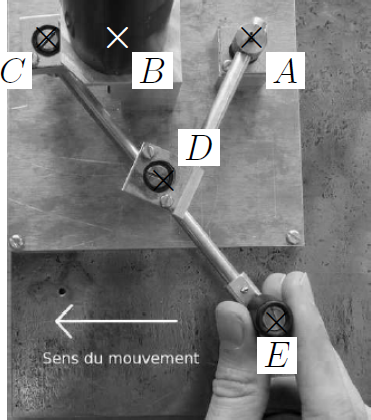
\includegraphics[width=\linewidth]{fig_00.png}
%\caption{Sous-système SEIS \label{fig_01}}
\end{marginfigure}


Le système étudié dans ce sujet est une tête de coupe de tissus conçue et réalisée par la société française Lectra, leader mondial dans la découpe automatisée des tissus.

\pargraph*{Présentation générale}

Un système de découpe automatisé de tissus est composé (figure \ref{fig_01}) :
\begin{itemize}
\item d’une table de découpe sur laquelle le tissus à découper (appelé matelas) est maintenu en position par aspiration ;
\item d’un bras transversal qui se déplace en translation de direction $\vy{0}$ par rapport à la table ;
\item d’une tête de coupe qui se déplace en translation de direction $\vx{0}$ par rapport au bras transversal ;
\item d’un ordinateur qui pilote l’ensemble du système.	 
\end{itemize}

\begin{marginfigure}
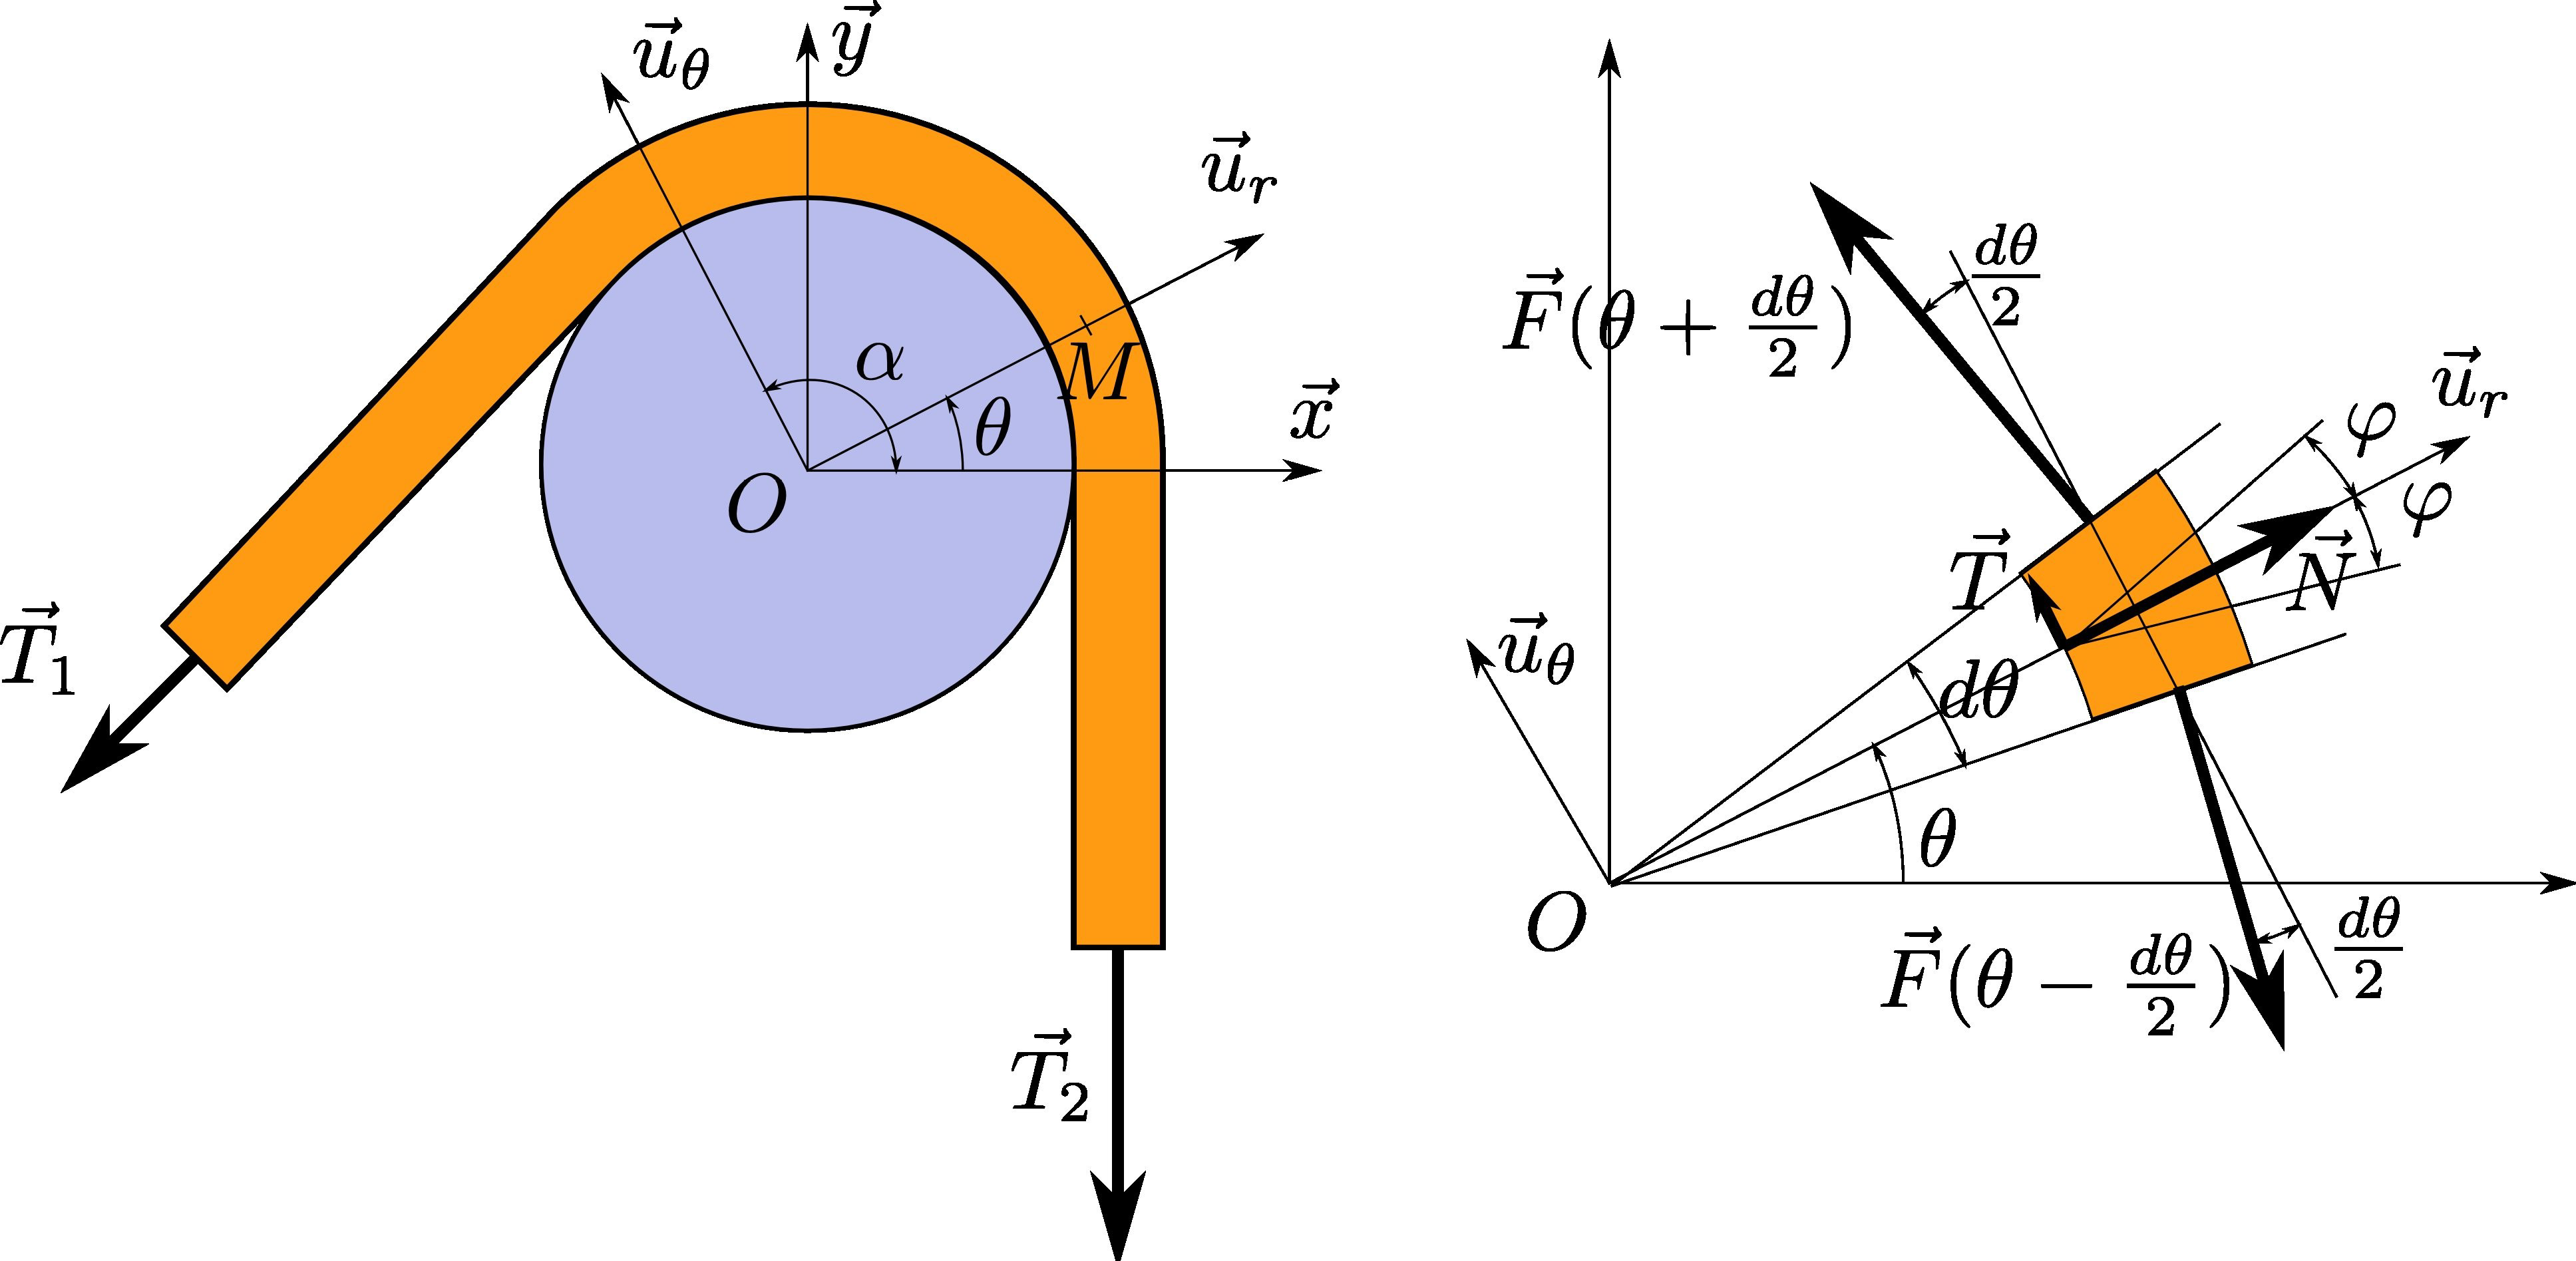
\includegraphics[width=\linewidth]{fig_01.png}
\caption{Structure d’une table de découpe de tissus \label{fig_01}}
\end{marginfigure}
	
Dans ce sujet, nous nous intéresserons plus particulièrement à la tête de coupe proposée par Lectra dans deux versions (initiale et améliorée) dont le diagramme partiel des exigences pour la solution de découpe (logiciel/machine) est présenté dans la figure \ref{fig_02}.


\begin{marginfigure}
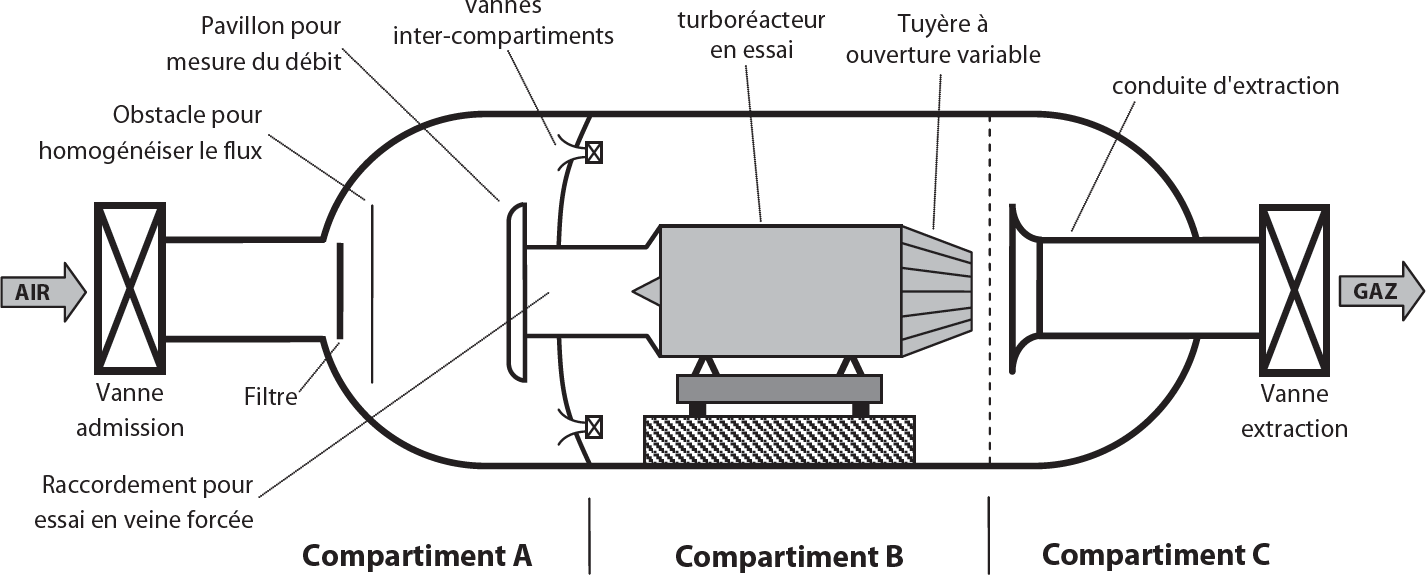
\includegraphics[width=\linewidth]{fig_02.png}
\caption{Diagramme des exigences \label{fig_02}}
\end{marginfigure}